\documentclass{standalone}
\usepackage{amsfonts,amsmath,amssymb}
\usepackage[slovene]{babel}
\usepackage[utf8]{inputenc}
\usepackage[T1]{fontenc}
  
\usepackage{tikz, verbatim}
\usepackage{pgfplots}
\usetikzlibrary{arrows.meta, calc, positioning, automata}

\begin{document}

	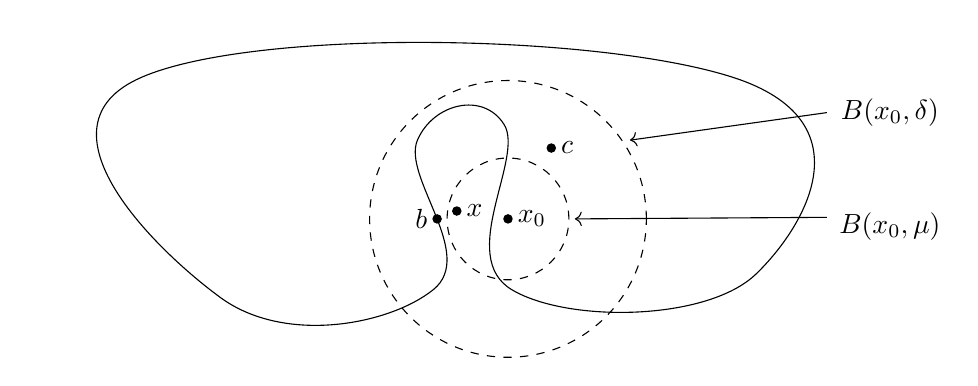
\begin{tikzpicture}
		\draw[black] plot [smooth cycle, tension = 0.8] coordinates {(-4, 2)  (3.5, 2) (3.8, -0.5) (0.7, -0.7) (0.6, 1.4) (-0.5, 1.2)  (-0.3, -0.7) (-3, -0.8)};
%		\filldraw[black] (-4, 2) circle (1.5pt);
%		\filldraw[black] (3.5, 2) circle (1.5pt);
%		\filldraw[black] (3.8, -0.5) circle (1.5pt);
%		\filldraw[black] (0.7, -0.7) circle (1.5pt);
%		\filldraw[black] (0.6, 1.4) circle (1.5pt);
%		\filldraw[black] (-1, -0.5) circle (1.5pt);
%		\filldraw[black] (-2.8, -1) circle (1.5pt);
		\filldraw[black] (0.65, 0.2) circle (1.5pt) node[black,right] {$x_0$};
		\filldraw[black] (0, 0.3) circle (1.5pt) node[black, right] {$x$};
		\filldraw[black] (-0.25, 0.2) circle (1.5pt) node[black, left] {$b$};
		\filldraw[black] (1.2, 1.1) circle (1.5pt) node[black, right] {$c$};
		\draw[black, style = dashed] (0.65, 0.2) circle (22pt);
		\draw[black, style = dashed] (0.65, 0.2) circle (50pt);
		\draw[black, <-] (2.2, 1.2) -- (4.7, 1.55);
		\draw[black, <-] (1.5, 0.2) -- (4.7, 0.22);
		\node at (5.5, 1.55){$B(x_0, \delta)$};
		\node at (5.5, 0.1){$B(x_0, \mu)$};
	\end{tikzpicture}
	
\end{document}